%%*****************************************************************************
%% DHBW Mannheim LaTeX-Vorlage für Projekt-, Studien- und Bachelorarbeiten 
%%
%% Autor: Tobias Dreher, Yves Fischer
%% Datum: 06.07.2011
%%
%% Autor: Michael Gruben
%% Datum: 15.05.2013
%%
%% Autor: Markus Barthel
%% Datum: 22.08.2014
%%
%% Autor: Kasimir Weilandt
%% Datum: 16.08.2023
%%*****************************************************************************

%!TEX root = ../dokumentation.tex

%
% Almost all settings can be set here
%

\RequirePackage[l2tabu, orthodox]{nag}	% weist in Commandozeile bzw. log auf veraltete LaTeX Syntax hin

\documentclass[%
	pdftex,
	oneside,						% onesided print
	12pt,							% fontsize
	parskip=half,					% half a line between paragraphs
	%	topmargin = 10pt,				% distance page margin (Std:1in) to header [according to log: unused]
	headheight = 12pt,				% height of header
	% 	headsep = 30pt,					% distance between header and text body [according to log: unused]
	headsepline,					% line after header
	footsepline,					% line before footer
	footheight = 16pt,				% height of footer
	abstract,						% abstract heading
	DIV=calc,						% calculates type area
	BCOR=8mm,						% binding correction left: 8mm
	headinclude=false,				% do not include header in type area calculation
	footinclude=false,				% do not include footer in type area calculation
	listof=totoc,					% display list of figures/tables in toc
	toc=bibliography,				% display bibliography in toc
]{scrreprt}							% Koma-Script report class, for longer bachelor thesis alternatively use scrbook


%%%%%%%%%%%%%%%%%%%%%%%%%%%
%% TEMPLATE SETTINGS
%%%%%%%%%%%%%%%%%%%%%%%%%%%
\newcommand{\einstellung}[1]{%
	\expandafter\newcommand\csname #1\endcsname{}
	\expandafter\newcommand\csname setze#1\endcsname[1]{\expandafter\renewcommand\csname#1\endcsname{##1}}
}
\newcommand{\langstr}[1]{\einstellung{lang#1}}

\einstellung{matrikelnr}
\einstellung{titel}
\einstellung{kurs}
\einstellung{datumAbgabe}
\einstellung{firma}
\einstellung{firmenort}
\einstellung{abgabeort}
\einstellung{abschluss}
\einstellung{studiengang}
\einstellung{dhbw}
\einstellung{betreuer}
\einstellung{gutachter}
\einstellung{zeitraum}
\einstellung{arbeit}
\einstellung{autor}
\einstellung{sprache}
\einstellung{schriftart}
\einstellung{seitenrand}
\einstellung{kapitelabstand}
\einstellung{spaltenabstand}
\einstellung{zeilenabstand}
\einstellung{zitierstil} 	% available settings
%%%%%%%%%%%%%%%%%%%%%%%%%%%%%%%%%%%%%%%%%%%%%%%%%%%%%%%%%%%%%%%%%%%%%%%%%%%%%%%
%                                   Einstellungen
%
% Hier können alle relevanten Einstellungen für diese Arbeit gesetzt werden.
% Dazu gehören Angaben u.a. über den Autor sowie Formatierungen.
%
%
%%%%%%%%%%%%%%%%%%%%%%%%%%%%%%%%%%%%%%%%%%%%%%%%%%%%%%%%%%%%%%%%%%%%%%%%%%%%%%%


%%%%%%%%%%%%%%%%%%%%%%%%%%%%%%%%%%%% Sprache %%%%%%%%%%%%%%%%%%%%%%%%%%%%%%%%%%%
%% Aktuell sind Deutsch und Englisch unterstützt.
%% Es werden nicht nur alle vom Dokument erzeugten Texte in
%% der entsprechenden Sprache angezeigt, sondern auch weitere
%% Aspekte angepasst, wie z.B. die Anführungszeichen und
%% Datumsformate.
\setzesprache{de} % oder en
%%%%%%%%%%%%%%%%%%%%%%%%%%%%%%%%%%%%%%%%%%%%%%%%%%%%%%%%%%%%%%%%%%%%%%%%%%%%%%%%

%%%%%%%%%%%%%%%%%%%%%%%%%%%%%%%%%%% Angaben  %%%%%%%%%%%%%%%%%%%%%%%%%%%%%%%%%%%
%% Die meisten der folgenden Daten werden auf dem
%% Deckblatt angezeigt, einige auch im weiteren Verlauf
%% des Dokuments.
\setzematrikelnr{1234510}
\setzekurs{ABC2008DE}
\setzetitel{In der Regel haben wir einen zweizeiligen Titel}
\setzedatumAbgabe{August 2011}
\setzefirma{Firma GmbH}
\setzefirmenort{Firmenort}
\setzeabgabeort{Abgabeort}
\setzeabschluss{Bachelor of Science}
\setzestudiengang{Cyber Security}
\setzedhbw{Mannheim}
\setzebetreuer{Dipl.-Ing.~(FH) Peter Pan}
\setzegutachter{Dr.\ Silvana Koch-Mehrin}
\setzezeitraum{12 Wochen}
\setzearbeit{Projektarbeit}
\setzeautor{Vorname Nachname}
%%%%%%%%%%%%%%%%%%%%%%%%%%%%%%%%%%%%%%%%%%%%%%%%%%%%%%%%%%%%%%%%%%%%%%%%%%%%%%%%

%%%%%%%%%%%%%%%%%%%%%%%%%%%% Literaturverzeichnis %%%%%%%%%%%%%%%%%%%%%%%%%%%%%%
%% Bei Fehlern während der Verarbeitung bitte in ads/header.tex bei der
%% Einbindung des Pakets biblatex (ungefähr ab Zeile 110,
%% einmal für jede Sprache), biber in bibtex ändern.
\newcommand{\ladeliteratur}{%
	\addbibresource{bibliographie.bib}
	%\addbibresource{weitereDatei.bib}
}
%% Zitierstil
%% siehe: http://ctan.mirrorcatalogs.com/macros/latex/contrib/biblatex/doc/biblatex.pdf (3.3.1 Citation Styles)
%% mögliche Werte z.B numeric-comp, alphabetic, authoryear
\setzezitierstil{numeric-comp}
%%%%%%%%%%%%%%%%%%%%%%%%%%%%%%%%%%%%%%%%%%%%%%%%%%%%%%%%%%%%%%%%%%%%%%%%%%%%%%%%

%%%%%%%%%%%%%%%%%%%%%%%%%%%%%%%%% Layout %%%%%%%%%%%%%%%%%%%%%%%%%%%%%%%%%%%%%%%
%% Verschiedene Schriftarten
% laut nag Warnung: palatino obsolete, use mathpazo, helvet (option scaled=.95), courier instead
\setzeschriftart{lmodern} % palatino oder goudysans, lmodern, libertine

%% Paket um Textteile drehen zu können
%\usepackage{rotating}
%% Paket um Seite im Querformat anzuzeigen
%\usepackage{lscape}

%% Seitenränder
\setzeseitenrand{2.5cm}

%% Abstand vor Kapitelüberschriften zum oberen Seitenrand
\setzekapitelabstand{20pt}

%% Spaltenabstand
\setzespaltenabstand{10pt}
%%Zeilenabstand innerhalb einer Tabelle
\setzezeilenabstand{1.5}
%%%%%%%%%%%%%%%%%%%%%%%%%%%%%%%%%%%%%%%%%%%%%%%%%%%%%%%%%%%%%%%%%%%%%%%%%%%%%%%%

%%%%%%%%%%%%%%%%%%%%%%%%%%%%% Verschiedenes  %%%%%%%%%%%%%%%%%%%%%%%%%%%%%%%%%%%
%% Farben (Angabe in HTML-Notation mit großen Buchstaben)
\newcommand{\ladefarben}{%
	\definecolor{LinkColor}{HTML}{00007A}
	\definecolor{ListingBackground}{HTML}{FCF7DE}
}
%% Mathematikpakete benutzen (Pakete aktivieren)
%\usepackage{amsmath}
%\usepackage{amssymb}

%% Programmiersprachen Highlighting (Listings)
\newcommand{\listingsettings}{%
	\lstset{%
		language=Java,			% Standardsprache des Quellcodes
		numbers=left,			% Zeilennummern links
		stepnumber=1,			% Jede Zeile nummerieren.
		numbersep=5pt,			% 5pt Abstand zum Quellcode
		numberstyle=\tiny,		% Zeichengrösse 'tiny' für die Nummern.
		breaklines=true,		% Zeilen umbrechen wenn notwendig.
		breakautoindent=true,	% Nach dem Zeilenumbruch Zeile einrücken.
		postbreak=\space,		% Bei Leerzeichen umbrechen.
		tabsize=2,				% Tabulatorgrösse 2
		basicstyle=\ttfamily\footnotesize, % Nichtproportionale Schrift, klein für den Quellcode
		showspaces=false,		% Leerzeichen nicht anzeigen.
		showstringspaces=false,	% Leerzeichen auch in Strings ('') nicht anzeigen.
		extendedchars=true,		% Alle Zeichen vom Latin1 Zeichensatz anzeigen.
		captionpos=b,			% sets the caption-position to bottom
		backgroundcolor=\color{ListingBackground}, % Hintergrundfarbe des Quellcodes setzen.
		xleftmargin=0pt,		% Rand links
		xrightmargin=0pt,		% Rand rechts
		frame=single,			% Rahmen an
		frameround=ffff,
		rulecolor=\color{darkgray},	% Rahmenfarbe
		fillcolor=\color{ListingBackground},
		keywordstyle=\color[rgb]{0.133,0.133,0.6},
		commentstyle=\color[rgb]{0.133,0.545,0.133},
		stringstyle=\color[rgb]{0.627,0.126,0.941}
	}
}
%%%%%%%%%%%%%%%%%%%%%%%%%%%%%%%%%%%%%%%%%%%%%%%%%%%%%%%%%%%%%%%%%%%%%%%%%%%%%%%%

%%%%%%%%%%%%%%%%%%%%%%%%%%%%%%%% Eigenes %%%%%%%%%%%%%%%%%%%%%%%%%%%%%%%%%%%%%%%
%% Hier können Ergänzungen zur Präambel vorgenommen werden (eigene Pakete, Einstellungen) 				% read settings
\newcommand{\iflang}[2]{%
	\IfStrEq{\thesislanguage}{#1}{#2}{}
}

\langstr{coverclosinginstructions}
\langstr{articlecourseofstudies}
\langstr{courseofstudies}
\langstr{atthedh}
\langstr{by}
\langstr{cstimeofproject}
\langstr{csstudentid}
\langstr{cscourse}
\langstr{cscompany}
\langstr{cssupervisor}
\langstr{csreviewer}
\langstr{confidentiallitynotice}
\langstr{authordeclaration}
\langstr{glossary}
\langstr{acronyms}
\langstr{abstract}
\langstr{appendix}
\langstr{listingname}
\langstr{listlistingname}
\langstr{listingautorefname} 				% available strings
\input{lang/\sprache} 				% read translations


%%%%%%%%%%%%%%%%%%%%%%%%%%%
%% LANGUAGE SETTINGS
%%%%%%%%%%%%%%%%%%%%%%%%%%%
\usepackage{xstring}
\usepackage[utf8]{inputenc}
\usepackage[T1]{fontenc}
% setting for the language of the package babel and the directory headings
\iflang{de}{\usepackage[main=ngerman, english]{babel}}
\iflang{en}{\usepackage[main=english, ngerman]{babel}}
\usepackage[autostyle=true,babel=true]{csquotes}


%%%%%%%%%%%%%%%%%%%%%%%%%%%
%% IMPORTS
%%%%%%%%%%%%%%%%%%%%%%%%%%%
\usepackage[a4paper, margin=\seitenrand,foot=1cm]{geometry}	% Margins and spacing
\usepackage[activate, stretch=10, shrink=10, kerning=true]{microtype}
\usepackage[onehalfspacing]{setspace}
\usepackage{makeidx}
\usepackage{longtable}
\usepackage{enumitem}				% more options for enumerations
\usepackage{graphicx}
\usepackage{pdfpages}   			% to include pdfs
\usepackage{xcolor} 				% for HTML notation
\usepackage{array}
\usepackage{calc}					% to calculate (picture table in cover sheet)
\usepackage[right]{eurosym}
\usepackage{wrapfig}
\usepackage{pgffor} 				% for automatic inclusion of chapters
\usepackage[perpage, hang, multiple, stable]{footmisc}	% footnotes
\usepackage[printonlyused]{acronym} % if desired, the footnote option can be inserted, in which case the explanation is not displayed inline but in a footnote
\usepackage{tocbasic}
\usepackage{listings}
\usepackage{scrhack}				% helps against some warnings
%\usepackage{showframe}				% for debugging the layout



%%%%%%%%%%%%%%%%%%%%%%%%%%%
%% CONFIGURATION
%%%%%%%%%%%%%%%%%%%%%%%%%%%
%%%%%%%% Mycrotype %%%%%%%%
\SetExtraKerning[unit=space]{
encoding={*},
family={bch},
series={*},
size={footnotesize,small,normalsize}
}{
\textendash={400,400},      		% en-dash, add more space around it
"28={ ,150},                		% left bracket, add space from right
"29={150, },                		% right bracket, add space from left
\textquotedblleft={ ,150},  		% left quotation mark, space from right
\textquotedblright={150, }  		% right quotation mark, space from left
}

% Notes. Usage with \todo{note} or \todo[inline]{note}.
\usepackage[obeyFinal,backgroundcolor=yellow,linecolor=black]{todonotes}
% Hide all notes with the option "final" in \documentclass[...] or by commenting out the following line
% \usepackage[disable]{todonotes}

% Comment environment. Usage with \comment{}. Hide all comments by commenting the following line and activating the next line.
\newcommand{\comment}[1]{\par {\bfseries \color{blue} #1 \par}} % view comments		
% \newcommand{\comment}[1]{} % hide all comments

%% Apply font settings
\usepackage{\schriftart}
\ladefarben{}

% Title, author and date
\title{\titel}
\author{\autor}
\date{\datum}

%%%%%%%% Hyperref %%%%%%%%
% PDF settings
\usepackage[
	pdftitle={\titel},
	pdfauthor={\autor},
	pdfsubject={\arbeit},
	pdfcreator={pdflatex, LaTeX with KOMA-Script},
	pdfpagemode=UseOutlines, 		% display table of contents on opening
	pdfdisplaydoctitle=true, 		% display document title instead of file name in title bar
	pdflang={\sprache}, 			% language of the document
	hidelinks,
]{hyperref}

% (color-)settings for links in the pdf
\hypersetup{%
	colorlinks=true, 				% activate colored links
	linkcolor=LinkColor, 			% set color
	citecolor=LinkColor,
	filecolor=LinkColor,
	menucolor=LinkColor,
	urlcolor=LinkColor,
	bookmarksnumbered=true 			% show chapter numbers in pdf bookmarks
}
% Workaround to solve bug in Hyperref, must stay here
\usepackage{bookmark} 				% only one latex run is needed to update table of contents and references		

% a little bit smaller fonts in captions
\addtokomafont{caption}{\small}

%%%%%%%% BIBLATEX %%%%%%%%%
% literature references
\iflang{de}{%
	\usepackage[
		backend=biber,				% recommended. If biber causes problems: bibtex
		bibwarn=true,
		bibencoding=utf8,			% if .bib is utf8, otherwise ascii
		sortlocale=de_DE,
		style=\zitierstil,
	]{biblatex}
}
\iflang{en}{%
	\usepackage[
		backend=biber,				% recommended. If biber causes problems: bibtex
		bibwarn=true,
		bibencoding=utf8,			% if .bib is utf8, otherwise ascii
		sortlocale=en_US,
		style=\zitierstil,
	]{biblatex}
}

\ladeliteratur{}

% Glossar
\usepackage[nonumberlist,toc]{glossaries}

%%%%%% Additional Settings %%%%%%

% Hurenkinder und Schusterjungen verhindern
% prevent widow and orphan lines
\clubpenalty = 10000 				% prevent orphans (first line of a paragraph at the end of a page)
\widowpenalty = 10000 				% prevent widows  (last line of a paragraph at the beginning of a page)
\displaywidowpenalty=10000

% image path
\graphicspath{{images/}}

% some often used programming languages
\lstloadlanguages{PHP,Python,Java,C,C++,bash}
\listingsettings{}
% rename listings
\renewcommand\lstlistingname{\langlistingname}
\renewcommand\lstlistlistingname{\langlistlistingname}
\def\lstlistingautorefname{\langlistingautorefname}

% spacing in tables
\setlength{\tabcolsep}{\spaltenabstand}
\renewcommand{\arraystretch}{\zeilenabstand}

\makeglossaries
%!TEX root = ../dokumentation.tex

%
% vorher in Konsole folgendes aufrufen:
%	makeglossaries makeglossaries dokumentation.acn && makeglossaries dokumentation.glo
%

%
% Glossareintraege --> referenz, name, beschreibung
% Aufruf mit \gls{...}
%
\newglossaryentry{Glossareintrag}{name={Glossareintrag},plural={Glossareinträge},description={Ein Glossar beschreibt verschiedenste Dinge in kurzen Worten}}

\begin{document}

% Deckblatt
\begin{spacing}{1}
	%!TEX root = ../dokumentation.tex

%%**************************************************************
%% Credits: https://github.com/maxikoehler/LaTeX_DHBW-Mannheim
%%**************************************************************

% Deckblatt für Projektarbeiten
% Cover page for project theses

\begin{titlepage}
	\newgeometry{left=2.5cm,right=2.5cm,top=2cm,bottom=2.5cm}

	\begin{center}
		\begin{minipage}[]{0.49\textwidth}
			\begin{flushleft}
				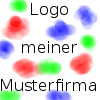
\includegraphics[width=2.5cm]{images/firmenlogo.png}
			\end{flushleft}
		\end{minipage}
		\begin{minipage}[]{0.49\textwidth}
			\begin{flushright}
				\includegraphics[width=3.9cm]{images/dhbw.png}
			\end{flushright}
		\end{minipage}
	\end{center}

	\enlargethispage{20mm}

	\begin{center}
		\vspace*{6mm}	{\thesistype}\\
		\doublespacing
		\vspace*{12mm}	{\LARGE\textbf{{\thesistitle}}}\\
		\onehalfspacing
		% \vspace*{12mm}	\includegraphics[width=16cm]{images/cover_sample.jpg}\\
		\vspace*{12mm}	für das 01. und 02. Theoriesemester (T3\_1000)\\
		\vspace*{3mm}		\langarticlecourseofstudies{} \langcourseofstudies{} \textbf{\coursesofstudies}\\
		\vspace*{3mm}		\langatthedh{} \dhbwcity\\
		\vspace*{7mm}	\langby\\
		\vspace*{3mm}		{\large\textbf \thesisauthor}\\
		\vspace*{7mm}	\submissiondate\\
	\end{center}

	\vfill

	\raggedleft
	\begin{spacing}{1.2}
		\begin{tabbing}
			mmmmmmmmmmmmmmmmmmmmmmmm              \= \kill
			\textbf{\langcstimeofproject} \> \timeperiod\\
			\textbf{\langcsstudentid, \langcscourse} \> \studentid, \course\\
			\textbf{\langcscompany} \> \company\\
			\> \companylocation\\
			\textbf{\langcssupervisor} \> \supervisor\\
			% \textbf{\langcsreviewer}              \>  \reviewer\\
		\end{tabbing}
	\end{spacing}
	\vspace{1cm}

	\vspace{1cm}
	\restoregeometry
\end{titlepage}

\end{spacing}
\newpage

\pagenumbering{Roman}

% Sperrvermerk
% %!TEX root = ../dokumentation.tex

\thispagestyle{empty}
% Sperrvermerk direkt hinter Titelseite
% Confidentiality notice right behind the title page
% https://www.mannheim.dhbw.de/fileadmin/user_upload/Studienangebot/Technik/__Downloads/Leitlinien-fuer-Bearbeitung-und-Dokumentation-FKT-DHBW-201909.pdf
\section*{\langsperrvermerk}

\vspace*{2em}

\iflang{de}{%
	Die vorliegende {\arbeit} 
	\begin{center}{\itshape{} \titel{}\/}\end{center} 
	enthält interne bzw. vertrauliche Daten der {\firma}.
	Sie ist ausschließlich zur Einsicht durch den zugewiesenen Prüfer, den Leiter des {\studiengang}-Fachbereichs und, falls notwendig, den Prüfungsausschuss \langanderdh{} {\dhbw} bestimmt.
	Es ist strengstens verboten
	\begin{itemize}
		\item den Inhalt dieser Arbeit (einschließlich Daten, Abbildungen, Tabellen, Diagramme etc.) ganz oder in Auszügen zu verbreiten,
		\item Kopien oder Abschriften dieser Arbeit oder von Teilen davon zu machen,
		\item diese Arbeit in digitaler, elektronischer oder virtueller Form zu verbreiten oder zugänglich zu machen.
	\end{itemize}
	Ausnahmefälle können durch eine schriftliche Genehmigung des Autors und der {\firma} berücksichtigt werden.
}

\iflang{en}{%
	The {\arbeit} on hand 
	\begin{center}{\itshape{} \titel{}\/}\end{center} 
	contains internal resp.\ confidential data of {\firma}. It is intended solely for inspection by the assigned examiner, the head of the {\studiengang} department and, if necessary, the Audit Committee \langanderdh{} {\dhbw}.
	It is strictly forbidden
	\begin{itemize}
		\item to distribute the content of this paper (including data, figures, tables, charts etc.) as a whole or in extracts,
		\item to make copies or transcripts of this paper or of parts of it,
		\item to display this paper or make it available in digital, electronic or virtual form.
	\end{itemize}
	Exceptional cases may be considered through permission granted in written form by the author and {\firma}.
}

\vspace{3em}

\abgabeort, \datumAbgabe
\vspace{4em}

\rule{6cm}{0.4pt}\\
\autor

% \newpage

% Erklärung
%!TEX root = ../dokumentation.tex

\thispagestyle{empty}

\section*{\langauthordeclaration}
\vspace*{2em}

% LTex: language=de-de
\iflang{de}{
	\begin{center}
		\begin{tabular}{| p{0.95\textwidth} |}
			\hline
			Ich versichere hiermit, dass ich meine \thesistype~mit dem Thema \glqq{\itshape \thesistitle }\grqq~selbstständig verfasst und keine anderen als die angegebenen Quellen und Hilfsmittel benutzt habe. \\
			Ich versichere zudem, dass die eingereichte elektronische Fassung mit der gedruckten Fassung übereinstimmt.*                                                                                           \\
			\footnotesize{\emph{*Falls beide Fassungen gefordert sind}}                                                                                                                                            \\
			\vspace{.5cm}
			Mannheim, den \submissiondate                                                                                                                                                                          \\
			\vspace*{.5cm}
			\singlespacing
			\rule{7cm}{.5pt}                                                                                                                                                                                       \\
			\thesisauthor                                                                                                                                                                                          \\[12pt]
			\hline
		\end{tabular}
	\end{center}

	\vfill

	%%%% Gender-Disclaimer %%%%
	% \begin{flushright}
	%     \begin{minipage}[]{0.8\textwidth}
	%         \raggedright
	%         \textbf{Hinweis:}\\[6pt]
	%         In dieser \thesistype~wird aus Gründen der besseren Lesbarkeit das generische Maskulinum verwendet. Weibliche und anderweitige Geschlechteridentitäten werden dabei ausdrücklich mitgemeint, soweit dies für die Aussage erforderlich ist.
	%     \end{minipage}
	% \end{flushright}
}

% LTex: language=en-us
\iflang{en}{%
	Hereby I solemnly declare:
	\begin{enumerate}
		\item that this {\thesistype}, titled {\itshape \thesistitle } is entirely the product of my own scholarly work, unless otherwise indicated in the text or references, or acknowledged below;
		\item I have indicated the thoughts adopted directly or indirectly from other sources at the appropriate places within the document;
		\item this {\thesistype} has not been submitted either in whole or part, for a degree at this or any other university or institution;
		\item I have not published this {\thesistype} in the past;
		\item the printed version is equivalent to the submitted electronic one.
	\end{enumerate}
	I am aware that a dishonest declaration will entail legal consequences.
}
\newpage

% Abstract
%!TEX root = ../dokumentation.tex

\pagestyle{empty}

\iflang{de}{%
% Dieser deutsche Teil wird nur angezeigt, wenn die Sprache auf Deutsch eingestellt ist.
\renewcommand{\abstractname}{\langabstract} % Text für Überschrift

% \begin{otherlanguage}{english} % auskommentieren, wenn Abstract auf Deutsch sein soll
\begin{abstract}
Abstract normalerweise auf Englisch. Siehe:  \url{http://www.dhbw.de/fileadmin/user/public/Dokumente/Portal/Richtlinien_Praxismodule_Studien_und_Bachelorarbeiten_JG2011ff.pdf} (8.3.1 Inhaltsverzeichnis)

Ein "`Abstract"' ist eine prägnante Inhaltsangabe, ein Abriss ohne Interpretation und Wertung einer wissenschaftlichen Arbeit. In DIN 1426 wird das (oder auch der) Abstract als Kurzreferat zur Inhaltsangabe beschrieben.

\begin{description}
\item[Objektivität] soll sich jeder persönlichen Wertung enthalten
\item[Kürze] soll so kurz wie möglich sein
\item[Genauigkeit] soll genau die Inhalte und die Meinung der Originalarbeit wiedergeben
\end{description}

Üblicherweise müssen wissenschaftliche Artikel einen Abstract enthalten, typischerweise von 100-150 Wörtern, ohne Bilder und Literaturzitate und in einem Absatz.

Quelle: \url{http://de.wikipedia.org/wiki/Abstract} Abgerufen 07.07.2011

Diese etwa einseitige Zusammenfassung soll es dem Leser ermöglichen, Inhalt der Arbeit und Vorgehensweise
des Autors rasch zu überblicken. Gegenstand des Abstract sind insbesondere 
\begin{itemize}
\item Problemstellung der Arbeit,
\item im Rahmen der Arbeit geprüfte Hypothesen bzw. beantwortete Fragen,
\item der Analyse zugrunde liegende Methode,
\item wesentliche, im Rahmen der Arbeit gewonnene Erkenntnisse,
\item Einschränkungen des Gültigkeitsbereichs (der Erkenntnisse) sowie nicht beantwortete Fragen. 
\end{itemize}
Quelle: \url{http://www.ib.dhbw-mannheim.de/fileadmin/ms/bwl-ib/Downloads_alt/Leitfaden_31.05.pdf}, S.~49
\end{abstract}
% \end{otherlanguage} % auskommentieren, wenn Abstract auf Deutsch sein soll
}



\iflang{en}{%
% Dieser englische Teil wird nur angezeigt, wenn die Sprache auf Englisch eingestellt ist.
\renewcommand{\abstractname}{\langabstract} % Text für Überschrift

\begin{abstract}
An abstract is a brief summary of a research article, thesis, review, conference proceeding or any in-depth analysis of a particular subject or discipline, and is often used to help the reader quickly ascertain the paper's purpose. When used, an abstract always appears at the beginning of a manuscript, acting as the point-of-entry for any given scientific paper or patent application. Abstracting and indexing services for various academic disciplines are aimed at compiling a body of literature for that particular subject.

The terms précis or synopsis are used in some publications to refer to the same thing that other publications might call an ``abstract''. In ``management'' reports, an executive summary usually contains more information (and often more sensitive information) than the abstract does.

Quelle: \url{http://en.wikipedia.org/wiki/Abstract_(summary)}

\end{abstract}
}
\newpage

\pagestyle{plain}		% nur Seitenzahlen im Fuß

\RedeclareSectionCommand[beforeskip=\chapterspacing]{chapter} % stellt Abstand vor Kapitelüberschriften ein

{ % Lokale Umgebung um Links schwarz zu machen
	\hypersetup{
		linkcolor=black,
		% linktocpage=true, 		% Nicht der Text sondern die Seitenzahlen in Verzeichnissen klickbar
	}

	% Inhaltsverzeichnis
	\begin{spacing}{1.1}
		\begingroup

		% auskommentieren für Seitenzahlen unter Inhaltsverzeichnis
		\renewcommand*{\chapterpagestyle}{empty}
		\pagestyle{empty}


		\setcounter{tocdepth}{1}
		%für die Anzeige von Unterkapiteln im Inhaltsverzeichnis
		%\setcounter{tocdepth}{2}

		\tableofcontents
		\clearpage
		\endgroup
	\end{spacing}
	\newpage

	% Abkürzungsverzeichnis
	\cleardoublepage
	%!TEX root = ../dokumentation.tex

\addchap{\langabkverz}
% only used acronyms will be listed in the abbreviation list
% Usage:
%		\ac{abb.}	--> inserts the abbreviation; the first time it is called, the full version is also automatically inserted in front of it or displayed in a footnote (for this, \usepackage[printonlyused,footnote]{acronym} must be in header.tex)
%		\acs{abb.}	--> inserts the abbreviation
%		\acf{abb.}	--> inserts the abbreviation and the full version
%		\acl{abb.}	--> inserts only the full version
%		\acp{abb.}	--> outputs the plural form of the abbreviation (added 's'); the additional 'p' can also be used with all of the above commands
% see also: http://golatex.de/wiki/%5Cacronym
%
\begin{acronym}[YTMMM]
	\setlength{\itemsep}{-\parsep}

	\acro{AGPL}{Affero GNU General Public License}
	\acro{WSN}{Wireless Sensor Network}
	\acro{MANET}{Mobile wireless Ad-hoc NETwork}
	\acro{MAC}{Multiple Access Control}
	\acro{QoS}{Quality of Service}
	\acro{DSR}{Dynamic Source Routing}
	\acro{API}{Application Programming Interface}
	\acro{WYSIWYG}{What You See Is What You Get}
	\acro{HTML}{HyperText Markup Language}
\end{acronym}


	% Abbildungsverzeichnis
	\cleardoublepage
	\listoffigures

	%Tabellenverzeichnis
	\cleardoublepage
	\listoftables

	% Quellcodeverzeichnis
	\cleardoublepage
	\lstlistoflistings
	\cleardoublepage
}
\pagenumbering{arabic}

\pagestyle{headings}		% Kolumnentitel im Kopf, Seitenzahlen im Fuß

% Inhalt
\foreach \i in {01,02,03,04,05,06,07,08,09,...,99} {%
		\edef\FileName{content/\i chapter}%
		\IfFileExists{\FileName}{%
			\input{\FileName}
		}
		{%
			%file does not exist
		}
	}

\clearpage

% Literaturverzeichnis
\cleardoublepage
\printbibliography

% Glossar
\printglossary[style=altlist,title=\langglossary]

% sonstiger Anhang
\clearpage
\appendix
% !TeX root = ../dokumentation.tex

\addchap{\langappendix}

(Beispielhafter Anhang)


{\Large
	\begin{enumerate}[label=\Alph*.]
		\item Assignment
		\item List of CD Contents
		\item CD
	\end{enumerate}
}
\pagebreak
%\includepdf[pages=-,scale=.9,pagecommand={}]{Aufgabenstellung.pdf} % PDF um 10% verkleinert einbinden --> Kopf- und Fußzeile  werden so korrekt dargestellt. Die Option `pages' ermöglicht es, eine bestimmte Sequenz von Seiten (z.B. 2-10 oder `-' für alle Seiten) auszuwählen.
\pagebreak
\section*{B. List of CD Contents}
\begin{tabbing}
	mm \= mm \= mmmmmmmmmmmmmmmm \= \kill
	$\vdash$ \textbf{Literature/} \\
	| \> $\vdash$ \textbf{Citavi-Project(incl pdfs)/} \> \> $\Rightarrow$ \textit{Citavi (bibliography software) project with}\\
	| \> | \> \> \textit{almost all found sources relating to this report.} \\
	| \> | \> \> \textit{The PDFs linked to bibliography items therein} \\
	| \> | \> \> \textit{are in the sub-directory `CitaviFiles'}\\
	| \> | \>  -- bibliography.bib  \> $\Rightarrow$ \textit{Exported Bibliography file with all sources}\\
	| \> | \>  --	Studienarbeit.ctv4  \>  $\Rightarrow$ \textit{Citavi Project file}\\
	| \> | \>  $\vdash$ \textbf{CitaviCovers/} \>  $\Rightarrow$ \textit{Images of bibliography cover pages}\\
	| \> | \>  $\vdash$ \textbf{CitaviFiles/} \> $\Rightarrow$ \textit{Cited and most other found PDF resources}\\ %\llcorner
	| \> $\vdash$ \textbf{eBooks/} \\
	| \> $\vdash$ \textbf{JournalArticles/} \\
	| \> $\vdash$ \textbf{Standards/}\\
	| \> $\vdash$ \textbf{Websites/} \\ %\llcorner
	|\\
	$\vdash$ \textbf{Presentation/} \\
	| \>  --presentation.pptx\\
	| \>  --presentation.pdf\\
	|\\
	$\vdash$ \textbf{Report/} \\ %\llcorner
	\>  -- Aufgabenstellung.pdf\\
	\>  -- Studienarbeit2.pdf\\
	\>  $\vdash$ \textbf{Latex-Files/}   $\Rightarrow$ \textit{editable \LaTeX~files and other included files for this report}\\ %\llcorner
	\> \>  $\vdash$  \textbf{ads/}   	\> $\Rightarrow$ \textit{Front- and Backmatter}\\
	\> \>  $\vdash$  \textbf{content/}  \> $\Rightarrow$ \textit{Main part}\\
	\> \>  $\vdash$  \textbf{images/}   \> $\Rightarrow$ \textit{All used images}\\
	\> \>  $\vdash$  \textbf{lang/}  \> $\Rightarrow$ \textit{Language files for \LaTeX~template}\\ %\llcorner
\end{tabbing}

\end{document}